%_________________________________________________________________________________________

\chapter{Preliminaries}
\label{chap:preliminaries}

This chapter introduces the formal models and core definitions used throughout the thesis. We present \emph{negotiations} as our framework for modeling concurrency, and \emph{timed automata} as our reference model for quantitative time. Both models serve as building blocks for local-timed negotiations, which we introduce in Chapter~\ref{chap:ltn}.

All definitions presented here are standard or adapted from existing literature, particularly~\cite{EsparzaDeselNegotiations,AlurDillTA}. This chapter is purely foundational—no new results appear. The level of detail ensures that later constructions can be understood without consulting original sources.

\paragraph{Organization.} Section~\ref{sec:negotiations} introduces negotiations, their semantics, and key examples. Section~\ref{sec:timed-automata} recalls timed automata, region abstractions, and their decidability results. Section~\ref{sec:networks-ta} briefly covers networks of timed automata. Section~\ref{sec:summary} summarizes and previews the synthesis of these models in local-timed negotiations.

%_________________________________________________________________________________________

\section{Negotiations}
Negotiations provide an interaction-centric model of concurrency in which synchronization is explicit and causality is transparent; this makes them a natural substrate for studying the impact of timing and synchronization on reachability.

The formal model of distributed negotiations is inspired by van der Aalst’s workflow Petri nets~\cite{}. A negotiation consists of a collection of \emph{atomic negotiations} (also called atoms or nodes), each representing a synchronized interaction among a non-empty set of agents (also called processes). Each atom has a finite set of possible \emph{outcomes}, corresponding to the different ways in which the interaction may resolve.

Atoms are composed into a distributed negotiation by means of a \emph{next-atoms} function that determines, for each atom, each participating agent, and each outcome, the set of atoms that the agent is ready to engage in next if that outcome occurs. We assume that every negotiation has a distinguished initial atom involving all agents, which marks the start of the interaction.

In the original definition, outcomes are additionally equipped with state-transformers that update internal states of the participating agents. These internal states do not influence which atoms are enabled, and will be abstracted away later in this chapter, as we focus exclusively on the control-flow behaviour of negotiations.

Negotiations are particularly well-suited for modelling distributed workflows, business processes, and coordination protocols, and reveals structural properties that are not easily visible in state-based models. In particular, negotiations make synchronization explicit at the level of interactions, rather than encoding it indirectly via shared places or states, which leads to different structural and algorithmic properties.

%---------------------------------------------------------------------------------------------------------------------------------------------

\subsection{Syntax and Semantics}

We present negotiations in a control-flow-oriented form that abstracts away internal agent states. This abstraction suffices for reachability analysis, since internal states do not influence the enablement or ordering of atoms. The simplified model will later be extended with timing constraints in Chapter~\ref{chap:ltn}. Its relationship to the standard definition with transformers and internal states is discussed in Section~\ref{sec:standard-def}.

This is not a new model, but an abstraction of the standard one that preserves exactly the control-flow behaviour relevant for reachability.

\begin{definition}[Negotiation]
\label{def:negotiation}
Let $P$ be a finite set of \emph{agents} (or \emph{processes}), and $\S$ a finite set of \emph{outcomes}. A \textsf{negotiation} $\mathcal{N}$ is a tuple $(N, \text{dom}, \delta)$ where:
\begin{itemize}
\item $N$ is a finite set of \emph{nodes} (also called \emph{atoms} or \emph{atomic negotiations}),
\item $\text{dom} : N \rightarrow 2^P \setminus \{\emptyset\}$ maps each node to a non-empty subset of agents called its \emph{domain}; we assume $\text{dom}(n_{\text{in}}) = P$ for a distinguished \emph{initial node} $n_{\text{in}}$,
\item $\delta = \{\delta_p\}_{p \in P}$ is a tuple of transition relations, one per agent, where $\delta_p : N_p \times \S \rightarrow 2^{N_p}$ with $N_p = \{n \in N \mid p \in \text{dom}(n)\}$. For a node $n$ with outcome $r$, the set $\delta_p(n,r)$ specifies which nodes agent $p$ becomes ready for next if outcome $r$ occurs.
\end{itemize}
We call pairs $(n,r)$ with $n \in N$ and $r$ an outcome associated with $n$ the \emph{locations} of the negotiation.
\end{definition}

A node $n$ with $\text{dom}(n) = \{p,q,r\}$ represents a point where agents $p$, $q$, and $r$ must synchronize. Intuitively, an outcome represents a joint decision made by all participating agents when the node is fired. They jointly select an outcome $r$ from those available at $n$. Each agent $p \in \text{dom}(n)$ then transitions to a set of nodes $\delta_p(n,r)$, becoming ready to participate in any of those nodes next.

\paragraph{Semantics.}
A \emph{marking} $x : P \rightarrow 2^N$ records, for each agent, the set of nodes it is currently ready to participate in. The \emph{initial marking} $x_0$ satisfies $x_0(p) = \{n_{\text{in}}\}$ for all $p \in P$. A \emph{final marking} $x_f$ has $x_f(p) = \emptyset$ for all $p$, indicating termination.

A marking records, for each agent, the set of atoms it is currently ready to engage in. An atom $n$ is enabled exactly when all its participating agents are ready for it, i.e., when $n$ belongs to the readiness set of every agent in $dom(n)$. A node $n$ is \emph{enabled} in marking $x$ if $n \in x(p)$ for every $p \in \text{dom}(n)$—that is, all parties of $n$ are ready. When $n$ is enabled, its parties may agree on an outcome $r$; we say the \emph{outcome} $(n,r)$ \emph{occurs}. This produces a new marking $x'$ where:
\[
x'(p) = \begin{cases}
\delta_p(n,r) & \text{if } p \in \text{dom}(n), \\
x(p) & \text{otherwise}.
\end{cases}
\]
We write $x \xrightarrow{(n,r)} x'$ and call this a \emph{small step}.

\paragraph{Observation.} Note that for agents participating in the occurring atom, the previous set $x(p)$ is not preserved. That is, readiness is consumed rather than accumulated: after an occurrence $(n,r)$, an agent $p \in \dom(n)$ is ready exactly for the nodes in $\delta_p(n,r)$, and for no others. In contrast to Petri nets, readiness does not accumulate: for each agent, previous options are discarded when a new atom occurs.

A \emph{run} (or \emph{occurrence sequence}) from $x_0$ is a finite or infinite sequence:
\[
x_0 \xrightarrow{(n_1,r_1)} x_1 \xrightarrow{(n_2,r_2)} x_2 \xrightarrow{(n_3,r_3)} \cdots
\]
If the sequence ends at the final marking $x_f$, we call it a \emph{large step} or \emph{successful run}.

A marking that enables no node is a \emph{deadlock} (unless it is the final marking). A marking from which the final marking is unreachable, yet which can reoccur along some run, is a \emph{livelock}.

\begin{definition}[Reachability graph]
\label{def:reach-graph}
The \textsf{reachability graph} (or \textsf{marking graph}) of $\mathcal{N}$ has all markings reachable from $x_0$ as vertices. There is an arc from $x$ to $x'$ labeled $(n,r)$ whenever $x \xrightarrow{(n,r)} x'$. The initial marking $x_0$ is the distinguished initial vertex.
\end{definition}

\paragraph{Concurrency.} Two outcomes $(n_1,r_1)$ and $(n_2,r_2)$ enabled at the same marking $x$ are \emph{concurrent} if $\text{dom}(n_1) \cap \text{dom}(n_2) = \emptyset$. They can occur in any order; in particular, the resulting marking is the same. This captures true concurrency, not just interleaving.

\begin{definition}[Concurrent step reachability graph]
\label{def:concurrent-graph}
The \textsf{concurrent step reachability graph} has all reachable markings as vertices. An arc from $x$ to $x'$ is labeled by a non-empty set of pairwise concurrent outcomes $\{(n_1,r_1), \ldots, (n_k,r_k)\}$ if all are enabled at $x$ and their joint occurrence yields $x'$. Initial vertex is $x_0$.
\end{definition}

%---------------------------------------------------------------------------------------------------------------------------------------------

\subsection{Graphical Representation}

Negotiations admit an intuitive graphical representation. Each node $n$ appears as a thick black horizontal bar. For each agent $p \in \text{dom}(n)$, a white circle (a \emph{port}) is drawn on the bar. Outcomes are represented by labeled arrows leaving the ports.

A transition $\delta_p(n,r) = \{n_1, \ldots, n_k\}$ is drawn as a \emph{hyperarc}: an arrow labeled $r$ that branches from the port of $p$ at $n$ to the ports of $p$ at $n_1, \ldots, n_k$. If $k = 1$ (deterministic case), it is a simple arrow. If $k > 1$, the branching represents non-determinism in the control flow.

Markings are represented by placing tokens (black dots) at the branching points of hyperarcs, or in the middle of arcs when no branching exists.

%---------------------------------------------------------------------------------------------------------------------------------------------

\subsection{Reachability and Complexity}
\label{sec:reachability}

The \emph{reachability problem} for negotiations asks: given a negotiation $\mathcal{N}$ and a marking $x_{\text{target}}$, does there exist a run from $x_0$ reaching $x_{\text{target}}$? This problem is central to verification, as it captures safety properties (can bad states be reached?), deadlock-freedom (are deadlocks reachable?), and many liveness requirements.

%---------------------------------------------------------------------------------------------------------------------------------------------

\subsection{A Running Example: ATM Transaction}
\label{sec:running-example}

We introduce a small running example that will recur throughout the thesis to illustrate models and constructions. It builds on the ATM example introduced in Chapter~\ref{chap:intro}, but focuses on a different interaction scenario (PIN change rather than cash withdrawal), allowing us to reuse the same agents while varying the control flow.

\paragraph{Scenario.} A customer ($c$) wishes to reset their ATM PIN using a one-time password (OTP) sent by their bank ($b$). The ATM machine ($a$) mediates the interaction. The protocol proceeds as follows: Initially, all agents are in the node $n_{in}$ node. They choose the outcome $st$ to start the transaction. Agents $a$ and $c$ go to node $n_1$ and $b$ goes to $n_2$.The customer gives her card details and requests for a PIN change in the ATM at  node $n_1$ by choosing the outcome $req$. At $n_2$, the ATM conveys this request to the bank and sends the details through the outcome $det$. The bank and the customer talk to each other at $n_3$, and $b$ sends an OTP to the customer through the outcome $s\_otp$. At $n_4$, the customer enters the OTP in the ATM. After entering the OTP, shown by the outcome $e\_otp$ the customer is ready to engage with the ATM either at $n_4$ or at $n_6$, represented by the non-deterministic arc leading to $n_4$ and $n_6$. The ATM talks to the bank at $n_5$ to check the OTP. If it matches, the ATM goes to $n_6$, otherwise it goes back to $n_4$.

\paragraph{Formal description.}
Let $P = \{c, a, b\}$ denote customer, ATM, and bank respectively, $N = \{n_{in}, n_0, \dots, n_6\}, \S = \{\mathsf{start} req, det, e\_otp, match, fail, g\_up\}$.

\textbf{Functions and domains of the nodes:}
\begin{itemize}
\item $n_{\text{in}}$ (initial): $\text{dom}(n_{\text{in}}) = \{c,a,b\}$
\item $n_1$ (request): $\text{dom}(n_1) = \{c,a\}$
\item $n_2$ (forward details): $\text{dom}(n_2) = \{a,b\}$
\item $n_3$ (send OTP): $\text{dom}(n_3) = \{c,b\}$
\item $n_4$ (enter OTP): $\text{dom}(n_4) = \{c,a\}$
\item $n_5$ (validate OTP): $\text{dom}(n_5) = \{a,b\}$
\item $n_6$ (completion): $\text{dom}(n_6) = \{c,a,b\}$
\end{itemize}

\textbf{Outcomes and transitions:}
\begin{itemize}
\item At $n_{\text{in}}$: outcome $\mathsf{start}$ leads all agents to their next nodes: \\
$\delta_c(n_{\text{in}}, \mathsf{start}) = \{n_1\}$, $\delta_a(n_{\text{in}}, \mathsf{start}) = \{n_1\}$, $\delta_b(n_{\text{in}}, \mathsf{start}) = \{n_2\}$.

\item At $n_1$: outcome $\mathsf{req}$ (request) leads: \\
$\delta_c(n_1, \mathsf{req}) = \{n_3\}$, $\delta_a(n_1, \mathsf{req}) = \{n_2\}$.

\item At $n_2$: outcome $\mathsf{det}$ (details) leads: \\
$\delta_a(n_2, \mathsf{det}) = \{n_4\}$, $\delta_b(n_2, \mathsf{det}) = \{n_3\}$.

\item At $n_3$: outcome $\mathsf{s\_otp}$ (send OTP) leads: \\
$\delta_c(n_3, \mathsf{s\_otp}) = \{n_4\}$, $\delta_b(n_3, \mathsf{s\_otp}) = \{n_5\}$.

\item At $n_4$: two outcomes are possible:
\begin{itemize}
\item $\mathsf{e\_otp}$ (enter OTP): $\delta_c(n_4, \mathsf{e\_otp}) = \{n_4, n_6\}$ (customer ready for retry or completion), $\delta_a(n_4, \mathsf{e\_otp}) = \{n_5\}$.
\item $\mathsf{g\_up}$ (give up): $\delta_c(n_4, \mathsf{g\_up}) = \{n_6\}$, $\delta_a(n_4, \mathsf{g\_up}) = \{n_6\}$.
\end{itemize}

\item At $n_5$: two outcomes:
\begin{itemize}
\item $\mathsf{match}$ (OTP correct): $\delta_a(n_5, \mathsf{match}) = \{n_6\}$, $\delta_b(n_5, \mathsf{match}) = \{n_6\}$.
\item $\mathsf{fail}$ (OTP incorrect): $\delta_a(n_5, \mathsf{fail}) = \{n_4\}$, $\delta_b(n_5, \mathsf{fail}) = \{n_5\}$ (bank loops, ATM returns to entry).
\end{itemize}

\item At $n_6$: outcome $\mathsf{end}$ leads all agents to termination: \\
$\delta_c(n_6, \mathsf{end}) = \emptyset$, $\delta_a(n_6, \mathsf{end}) = \emptyset$, $\delta_b(n_6, \mathsf{end}) = \emptyset$.
\end{itemize}

Figure~\ref{fig:ATM} shows the graphical representation of this negotiation.

\begin{figure}[t]
\centering
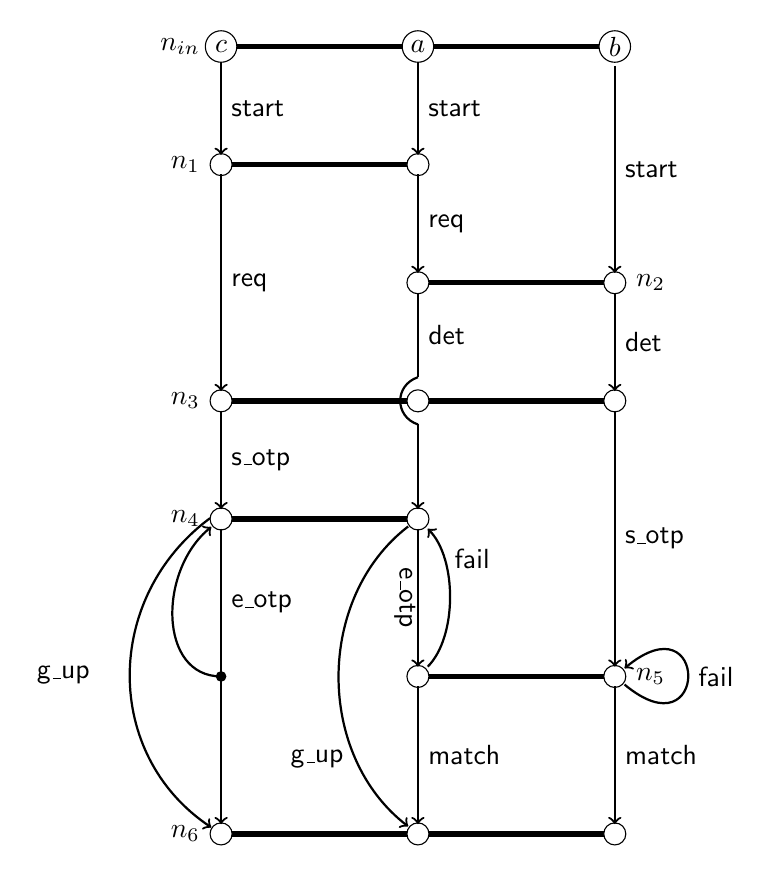
\begin{tikzpicture}

\begin{scope}[line width=2pt]
\draw (0.,0) node [left] {$n_{\text{in}}\,\,$} -- (5,0);
\draw (0.,-1.5) node [left] {$n_{1}\,\,$} -- (2.5,-1.5);
\draw (2.5,-3) -- (5,-3) node [right] {$\,\,n_{2}$};
\draw (0.,-4.5) node [left] {$n_{3}\,\,$} -- (5,-4.5);
\draw (0.,-6) node [left] {$n_{4}\,\,$} -- (2.5,-6);
\draw (2.5,-8) -- (5,-8)  node [right] {\,\,$n_{5}$};
\draw (0.,-10) node [left] {$n_{6}\,\,$} -- (5,-10);
\end{scope}

\begin{scope}[fill=white]
\filldraw  (0,0)  circle (2mm) node (nic) {$c$};
\filldraw  (2.5,0)  circle (2mm) node (nia) {$a$};
\filldraw  (5,0)  circle (2mm) node (nib) {$b$};

\filldraw  (0,-1.5)  circle (1.4mm) node (n1c) {};
\filldraw  (2.5,-1.5)  circle (1.4mm) node (n1a) {};

\filldraw  (2.5,-3)  circle (1.4mm) node (n2a) {};
\filldraw  (5,-3)  circle (1.4mm) node (n2b) {};

\filldraw  (0,-4.5)  circle (1.4mm) node (n3c) {};
\filldraw  (2.5,-4.5)  circle (1.4mm) node (n3a) {};
\filldraw  (5,-4.5)  circle (1.4mm) node (n3b) {};

\filldraw  (0,-6)  circle (1.4mm) node (n4c) {};
\filldraw  (2.5,-6)  circle (1.4mm) node (n4a) {};

\filldraw  (2.5,-8)  circle (1.4mm) node (n5a) {};
\filldraw  (5,-8)  circle (1.4mm) node (n5b) {};

\filldraw  (0,-10)  circle (1.4mm) node (n6c) {};
\filldraw  (2.5,-10)  circle (1.4mm) node (n6a) {};
\filldraw  (5,-10)  circle (1.4mm) node (n6b) {};

\filldraw  [fill=black] (0,-8)  circle (0.6mm) node (v1) {};
\end{scope}

\begin{scope}[thick,->]
\draw (nic) -- (n1c) node [right, midway] {$\mathsf{start}$};
\draw (n1c) -- (n3c) node [right, midway] {$\mathsf{req}$};
\draw (n3c) -- (n4c) node [right, midway] {$\mathsf{s\_otp}$};
\draw (n4c) -- (n6c) node [right, text width = 1.5 cm, near start] {$\mathsf{e\_otp}$};
\draw (0,-8) .. controls  (-0.8,-8) and (-0.8,-6.65) .. (n4c) node [left, midway] {};

\draw (nia) -- (n1a) node [right, midway] {$\mathsf{start}$};
\draw (n1a) -- (n2a) node [right, midway] {$\mathsf{req}$};
\draw (2.5,-4.8) -- (n4a);
\draw (n4a) -- (n5a) node [below=-0.1cm, sloped, midway] {$\mathsf{e\_otp}$};
\draw (n5a) -- (n6a) node [right, text width = 1 cm, midway] {$\mathsf{match}$};
\draw (n5a) .. controls (3,-7.5) and (3,-6.5) .. (n4a) node [right, near end] {$\mathsf{fail}$};
\draw (n4a) .. controls  (1.2,-7) and (1.2,-9) .. (n6a) node [left=-0.3cm, text width = 1 cm, near end] {$\mathsf{g\_up}$};

\draw (nib) -- (n2b) node [right, midway] {$\mathsf{start}$};
\draw (n2b) -- (n3b) node [right, midway] {$\mathsf{det}$};
\draw (n3b) -- (n5b) node [right, text width = 1 cm, midway] {$\mathsf{s\_otp}$};
\draw (n5b) -- (n6b) node [right, text width = 1 cm, midway] {$\mathsf{match}$};
\draw (n5b) .. controls  (6.2,-9) and (6.2,-7) .. (n5b) node [right, midway] {$\mathsf{fail}$};

\draw (n4c) + (-0.14,0.01) .. controls  (-1.5,-7) and (-1.5,-9) .. (n6c) node [left=-0.2cm, text width = 1.25 cm, midway] {$\mathsf{g\_up}$};
\end{scope}

\draw [thick] (n2a) -- (2.5,-4.2) node [right, midway] {$\mathsf{det}$};
\draw [thick] (2.5,-4.2) .. controls (2.2,-4.3) and (2.2,-4.7) .. (2.5,-4.8);
\end{tikzpicture}
\caption{ATM transaction negotiation. Customer ($c$), ATM ($a$), and bank ($b$) coordinate through atomic interactions. Note the hyperarc at $n_4$ for customer $c$ after $\mathsf{e\_otp}$: non-deterministic control flow allows readiness at both $n_4$ (retry) and $n_6$ (completion).}
\label{fig:ATM}
\end{figure}

\paragraph{Behavior.} Starting from $x_0$ where all agents are at $n_{\text{in}}$, outcome $\mathsf{start}$ occurs, moving $c$ and $a$ to $n_1$, and $b$ to $n_2$. Then $n_1$ and $n_2$ eventually both must occur before $n_3$ becomes enabled. The loop structure at $n_4 \to n_5 \to n_4$ models retry behavior when OTP validation fails. The customer can also ``give up" via outcome $\mathsf{g\_up}$, bypassing validation and proceeding directly to completion.

This example will reappear in Chapter~\ref{chap:ltn} when we add timing constraints to model, for instance, OTP expiration deadlines or maximum retry durations.

%---------------------------------------------------------------------------------------------------------------------------------------------

\subsection{Illustrative Examples: Control-Flow Patterns}

Before studying reachability and complexity, we present several examples highlighting non-trivial control-flow phenomena in negotiations. These patterns recur in distributed systems and will later interact with timing constraints in interesting ways.

%--------------------------------------------------------------------------

\subsubsection{Late Binding of Choice}
\label{subsec:neg-late-binding}

Negotiations allow choices made by a subset of agents to constrain future
interactions without being immediately resolved. This
\emph{late binding of choice}, is already illustrated by the pollination example~\ref{}
introduced in Chapter~\ref{chap:intro}. There, the outcome ($gc$ or $ch$) of the environment-related
node ($n_2$) determines whether normal ($n_4$) or early flowering ($n_5$) may occur later, even though
the agents participating in flowering do not take part in the climate decision.
Once the environment outcome is fixed, only the corresponding branch remains
feasible, and executions that mix incompatible branches are impossible.

Late binding of choice allows early, local decisions to propagate constraints
through the negotiation structure, with their effects realised only through
later multiparty interactions rather than immediate global synchronization.
This pattern will later reappear in local-timed negotiations~\ref{}, where relative timing
information accumulated early constrains which interactions are feasible later.
%--------------------------------------------------------------------------
\subsubsection{Example: Implicit Consensus}
\label{subsec:neg-implicit-consensus}

Negotiations can enforce agreement between agents through the structure of feasible
interactions, even in the absence of explicit communication or global
synchronization.

\begin{example}[Implicit consensus]
\label{ex:implicit-consensus}
Let $P=\{p,q,r\}$ and
\[
N=\{n_{pq},\, n_p,\, n_{qr}^0,\, n_{qr}^1,\, n_f\}.
\]
Domains are given by
\[
\dom(n_{pq})=\{p,q\},\quad \dom(n_p)=\{p\},\quad
\dom(n_{qr}^0)=\dom(n_{qr}^1)=\{q,r\},\quad \dom(n_f)=\{p,q,r\}.
\]
At $n_{pq}$ the set of outcomes is $\{0,1\}$. For $b\in\{0,1\}$, define
\[
\delta_p(n_{pq},b)=\{n_p\},\qquad
\delta_q(n_{pq},b)=\{n_{qr}^b\},\qquad
\delta_r(n_{pq},b)=\{n_{qr}^b\}.
\]
Node $n_p$ has a single outcome $x$ with $\delta_p(n_p,x)=\{n_f\}$.
Each node $n_{qr}^b$ has outcome $x$ with
\[
\delta_q(n_{qr}^b,x)=\{n_f\},\qquad
\delta_r(n_{qr}^b,x)=\{n_f\}.
\]
Finally, $n_f$ is terminal.
\end{example}

\paragraph{Observation.}
After the initial interaction at $n_{pq}$, agent $p$ never interacts again with
$q$ or $r$. Nevertheless, the outcome chosen at $n_{pq}$ uniquely determines which
interaction $q$ and $r$ must later execute: either $n_{qr}^0$ or $n_{qr}^1$.
Thus, $q$ and $r$ are forced to agree on a common branch, not through explicit
coordination or message-passing, but because all feasible continuations must be
consistent with the earlier choice. This example illustrates how negotiations can
enforce agreement purely via feasibility constraints—a phenomenon that will later
reappear when timing information is propagated and compared through selective
synchronization.

\subsubsection{Example: Transitive Causality Without Shared Participants}
\label{subsec:neg-causality-no-share}

Causality in negotiations is not restricted to interactions that share agents
directly; it can propagate transitively through the control-flow structure.

\begin{example}[Transitive causality]
\label{ex:causality-no-share}
Let $P=\{p,q,r,s\}$ and
\[
N=\{n_1,\, n_m,\, n_2\}
\]
with domains
\[
\dom(n_1)=\{p,q\},\quad \dom(n_m)=\{q,r\},\quad \dom(n_2)=\{r,s\}.
\]
All nodes have outcome $\{x\}$. Initially,
\[
x_0(p)=x_0(q)=\{n_1\},\qquad x_0(r)=x_0(s)=\emptyset.
\]
Transitions form a chain:
\begin{align*}
\delta_p(n_1,x) &= \emptyset, &
\delta_q(n_1,x) &= \{n_m\}, &
\delta_r(n_1,x) &= \{n_m\}, \\
\delta_q(n_m,x) &= \emptyset, &
\delta_r(n_m,x) &= \{n_2\}, &
\delta_s(n_m,x) &= \{n_2\}, \\
\delta_r(n_2,x) &= \emptyset, &
\delta_s(n_2,x) &= \emptyset.
\end{align*}
\end{example}

\paragraph{Observation.}
Although $\dom(n_1)\cap\dom(n_2)=\emptyset$, node $n_2$ cannot occur before $n_1$ in
any execution. The causal dependency $n_1 \prec n_2$ is transmitted through the
intermediate interaction $n_m$, which shares agents with both. This example shows
that causality in negotiations is a global, structural property rather than a
local one determined solely by shared participants. Such transitive dependencies
will play an important role later when timing constraints and synchronization
effects propagate along chains of interactions.

\begin{figure}[p] % 'p' places these on a separate page, 't' or 'h' for inline
\centering

% --- Example 2: Implicit Consensus ---
\begin{subfigure}[b]{0.45\textwidth}
\centering
\resizebox{\textwidth}{!}{%
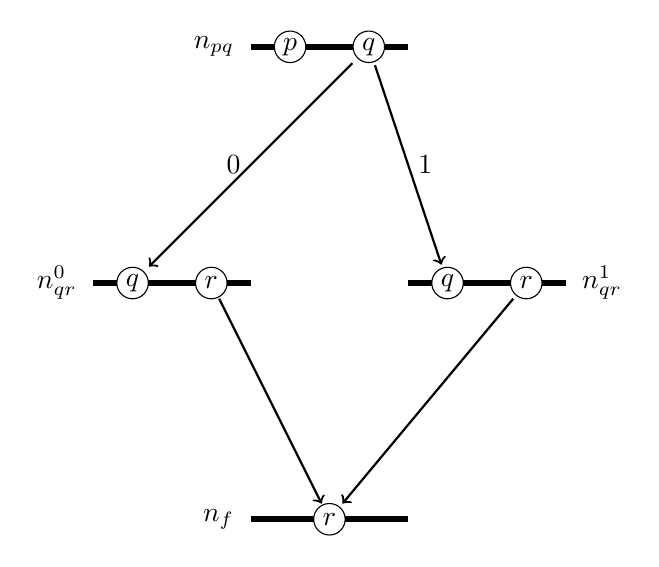
\begin{tikzpicture}
    % Nodes
    \draw[line width=2pt] (2,4) node[left] {$n_{pq}\,$} -- (4,4);
    
    \draw[line width=2pt] (0,1) node[left] {$n_{qr}^0\,$} -- (2,1);
    \draw[line width=2pt] (4,1) -- (6,1) node[right] {$\,n_{qr}^1$};
    
    \draw[line width=2pt] (2,-2) node[left] {$n_f\,$} -- (4,-2);

    % Ports
    \filldraw[fill=white] (2.5,4) circle (2mm) node (p_npq) {$p$};
    \filldraw[fill=white] (3.5,4) circle (2mm) node (q_npq) {$q$};
    
    \filldraw[fill=white] (0.5,1) circle (2mm) node (q_n0) {$q$};
    \filldraw[fill=white] (1.5,1) circle (2mm) node (r_n0) {$r$};
    
    \filldraw[fill=white] (4.5,1) circle (2mm) node (q_n1) {$q$};
    \filldraw[fill=white] (5.5,1) circle (2mm) node (r_n1) {$r$};
    
    \filldraw[fill=white] (3,-2) circle (2mm) node (r_nf) {$r$};

    % Edges
    \draw[->, thick] (q_npq) -- (q_n0) node[midway, left] {$0$};
    \draw[->, thick] (q_npq) -- (q_n1) node[midway, right] {$1$};
    
    \draw[->, thick] (r_n0) -- (r_nf);
    \draw[->, thick] (r_n1) -- (r_nf);
\end{tikzpicture}
}
\caption{\textbf{Implicit Consensus.} $q$ routes control based on $n_{pq}$, forcing $r$ to match.}
\label{fig:implicit_consensus}
\end{subfigure}

\vspace{1cm}

% --- Example 4: Transitive Causality ---
\begin{subfigure}[b]{0.45\textwidth}
\centering
\resizebox{\textwidth}{!}{%
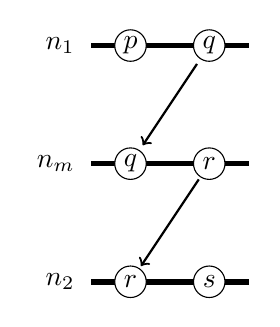
\begin{tikzpicture}
    % Nodes
    \draw[line width=2pt] (0,3) node[left] {$n_1\,$} -- (2,3);
    \draw[line width=2pt] (0,1.5) node[left] {$n_m\,$} -- (2,1.5);
    \draw[line width=2pt] (0,0) node[left] {$n_2\,$} -- (2,0);

    % Ports
    \filldraw[fill=white] (0.5,3) circle (2mm) node (p_n1) {$p$};
    \filldraw[fill=white] (1.5,3) circle (2mm) node (q_n1) {$q$};

    \filldraw[fill=white] (0.5,1.5) circle (2mm) node (q_nm) {$q$};
    \filldraw[fill=white] (1.5,1.5) circle (2mm) node (r_nm) {$r$};

    \filldraw[fill=white] (0.5,0) circle (2mm) node (r_n2) {$r$};
    \filldraw[fill=white] (1.5,0) circle (2mm) node (s_n2) {$s$};

    % Edges
    \draw[->, thick] (q_n1) -- (q_nm); % q flows n1 -> nm
    \draw[->, thick] (r_nm) -- (r_n2); % r flows nm -> n2
\end{tikzpicture}
}
\caption{\textbf{Transitive Causality.} $n_1 \prec n_2$ via shared agents $q,r$, despite disjoint domains.}
\label{fig:transitive_causality}
\end{subfigure}

\caption{Graphical representations of the control-flow examples discussed in Section~\ref{}.}
\label{fig:control_flow_examples}
\end{figure}

%---------------------------------------------------------------------------------------------------------------------------------------------

\subsection{Reachability and complexity results}
\label{sec:complexity}

We briefly summarize known complexity results for negotiations and related models. These results motivate both the use of negotiations as a concurrency formalism and the restrictions studied in later chapters.

\paragraph{General negotiations.}
For unrestricted negotiations, the reachability problem is decidable. However, the reachability graph can be exponential in the size of the negotiation, and several analysis problems are computationally expensive. In particular, soundness and reachability are PSPACE-hard in general.

\paragraph{Acyclic and sound negotiations.}
For important subclasses, the complexity drops significantly. For example, reachability and soundness are decidable in polynomial time for acyclic negotiations and for sound negotiations with restricted control-flow. These results contrast sharply with Petri nets, where even severely restricted classes often retain high complexity.

%add other results
%add 'timed negotiation' results
%---------------------------------------------------------------------------------------------------------------------------------------------

\subsection{Relation to Standard Negotiations with Transformers}
\label{sec:standard-def}

The negotiation model presented in Section~\ref{sec:negotiations} abstracts away internal agent states and transformers. For completeness and to connect with the original literature~\cite{EsparzaDeselNegotiations}, we briefly recall the standard definition and establish equivalence for control-flow properties. For the purposes of this thesis, the internal state evolution carried by transformers plays no role in enabling or disabling interactions.

\paragraph{Standard definition (informal).} In the original model, each agent $p$ has an internal state space $Q_p$ with initial states $Q_{0p}$. An atom $n$ involves parties $P_n$ and has outcomes $R_n$. Each outcome $r$ is associated with a \emph{transformer} $\tau_r$: a left-total relation $\tau_r \subseteq Q_A \times Q_A$ (where $Q_A = \prod_{p \in P} Q_p$) that is a $P_n$-transformer—it only affects states of agents in $P_n$.

When outcome $(n,r)$ occurs, agents in $P_n$ change states according to $\tau_r$, while agents outside $P_n$ remain unchanged. Crucially, \emph{enablement of an atom depends only on readiness}, not on the specific internal states of agents. The choice of outcome is non-deterministic and not restricted by internal states. Transformers determine only how internal states evolve \emph{after} an outcome occurs.

\paragraph{Why the simplification suffices.} Since this thesis focuses on reachability and control-flow properties, internal states are orthogonal: they do not influence which atoms are enabled or which outcomes can occur. All information relevant to reachability is captured by tracking which nodes each agent is ready for—exactly what markings record in our simplified definition.

\paragraph{Equivalence.}
The simplified definition of negotiations used in this thesis is equivalent to the standard definition with internal states and transformers, as far as reachability is concerned. Formally, from a standard negotiation one obtains the simplified model by projecting away internal states and retaining only the next-atom relation, which fully determines enablement and control flow. This simplification is semantic rather than approximate: it preserves the reachability graph exactly. Conversely, any simplified negotiation can be viewed as a standard one by equipping each agent with a trivial one-state internal domain and identity transformers. In both cases, the induced reachability graphs coincide. In both constructions, there is a bijection between reachable markings preserving enabled atoms and outcome occurrences. Occurrence sequences and reachability graphs correspond exactly. Properties expressible in terms of control flow (e.g., reachability, deadlock) are preserved.

%---------------------------------------------------------------------------------------------------------------------------------------------

\subsection{Relation to Petri Nets}
\label{sec:neg-pn}

Negotiations are closely related to a restricted class of Petri nets, and this
relationship is bidirectional. Esparza et al.~\cite{esparza-neg-pn,esparza-neg-ceur}
establish a behavior-preserving translation from negotiations to Petri nets and,
conversely, characterize negotiations as Petri nets satisfying strong structural
constraints.

\paragraph{From negotiations to Petri nets.}
Let $\mathcal{N}=(P,N,\dom,\delta,x_0)$ be a negotiation. One can construct a safe
Petri net $\mathcal{P}_{\mathcal{N}}=(\mathcal{P},\mathcal{T},F,M_0)$ as follows.
For each agent $p\in P$ and each atom $n\in N$ with $p\in\dom(n)$, the net contains a
place $(p,n)$ representing that agent $p$ is ready to engage in atom $n$. The initial
marking $M_0$ places one token in each place $(p,n)$ such that $n\in x_0(p)$.

For each outcome $(n,r)$ of an atom $n$, and for each choice of one input place
$(p,n)$ for every $p\in\dom(n)$, the net contains a transition $t_{n,r}$. The preset
of $t_{n,r}$ consists of the places $(p,n)$ for $p\in\dom(n)$, and its postset
consists of all places $(p,n')$ with $n'\in\delta_p(n,r)$. Firing $t_{n,r}$ consumes
one token from each input place and produces tokens according to the transition
function of the negotiation.

This construction preserves reachability: a marking is reachable in
$\mathcal{N}$ if and only if the corresponding marking is reachable in
$\mathcal{P}_{\mathcal{N}}$. Moreover, two outcomes are concurrently enabled in
$\mathcal{N}$ if and only if the corresponding transitions are independent in
$\mathcal{P}_{\mathcal{N}}$.

\paragraph{Structural characterization.}
The Petri nets obtained from negotiations satisfy strong restrictions. They are
safe, and their places are partitioned by agents, so that each token represents the
local control state of exactly one agent. Synchronization occurs only at transitions
whose preset contains exactly one place per participating agent. In particular,
tokens are never merged or split across agents, and no place is shared between
agents.

Conversely, Esparza et al.~\cite{esparza-neg-ceur} show that every Petri net satisfying
these structural conditions corresponds to a negotiation, in the sense that its
behavior can be captured by an interaction-centric model with atoms and outcomes.
Thus, negotiations form a well-defined fragment of safe workflow Petri nets in which
control flow is mediated exclusively by multiparty interactions.

\paragraph{Consequences.}
The restricted synchronization discipline of negotiations distinguishes them from
general Petri nets and underlies their improved algorithmic properties. These
structural features will be crucial when extending the model with local timing
constraints in later chapters.

%---------------------------------------------------------------------------------------------------------------------------------------------

\section{Timed Automata}
\label{sec:timed-automata}

Timed automata~\cite{AlurDillTA} extend finite automata with real-valued clock variables that evolve continuously with time. They provide the standard framework for modeling and verifying real-time systems, and form the semantic foundation for the timing aspects of local-timed negotiations.

We briefly recall their definition, operational semantics, and the region-based decidability result for reachability, which will serve as a conceptual template for later constructions. This material is standard; we include it to establish notation and to highlight which techniques transfer (or fail to transfer) to local-timed negotiations.

%---------------------------------------------------------------------------------------------------------------------------------------------

\subsection{Syntax and Semantics}

We work in dense time over the non-negative reals $\mathbb{R}_{\geq 0}$. All clocks evolve synchronously with global time in standard timed automata.

\paragraph{Clock constraints.} Let $X$ be a finite set of \emph{clocks}. A \emph{clock valuation} is a function $v : X \to \mathbb{R}_{\geq 0}$. For $\delta \in \mathbb{R}_{\geq 0}$, we write $v + \delta$ for the valuation $(v + \delta)(x) = v(x) + \delta$ (uniform time elapse). For $Y \subseteq X$, we write $[Y]v$ for the valuation that resets clocks in $Y$ to zero: $([Y]v)(x) = 0$ if $x \in Y$, and $([Y]v)(x) = v(x)$ otherwise.

The set of \emph{clock constraints} over $X$, denoted $\mathcal{C}(X)$, is defined by the grammar:
\[
g ::= x \bowtie c \mid g \wedge g
\]
where $x \in X$, $c \in \mathbb{N}$, and $\bowtie \in \{<, \leq, =, \geq, >\}$. A valuation $v$ \emph{satisfies} constraint $g$, written $v \models g$, if $g$ evaluates to true when each clock $x$ is replaced by $v(x)$.

\begin{definition}[Timed automaton]
\label{def:timed-automaton}
A \textsf{timed automaton} (TA) is a tuple $\mathcal{A} = (Q, \S, X, T, q_0, \text{Acc})$ where:
\begin{itemize}
\item $Q$ is a finite set of \emph{states} (or \emph{locations}),
\item $\S$ is a finite \emph{alphabet} of actions,
\item $X$ is a finite set of \emph{clocks},
\item $q_0 \in Q$ is the \emph{initial state},
\item $\text{Acc} \subseteq Q$ is the set of \emph{accepting states},
\item $T \subseteq Q \times \S \times \mathcal{C}(X) \times 2^X \times Q$ is a finite set of \emph{transitions}. A transition $(q, a, g, R, q') \in T$ has source state $q$, action label $a$, guard $g$, reset set $R$, and target state $q'$.
\end{itemize}
\end{definition}

\paragraph{Semantics.} The behavior of $\mathcal{A}$ is given by an infinite-state transition system whose \emph{configurations} are pairs $(q, v)$ consisting of a state $q \in Q$ and a valuation $v : X \to \mathbb{R}_{\geq 0}$. The \emph{initial configuration} is $(q_0, \mathbf{0})$ where $\mathbf{0}$ denotes the valuation assigning zero to all clocks.

There are two kinds of transitions:
\begin{itemize}
\item \textbf{Delay transitions:} $(q, v) \xrightarrow{\delta} (q, v + \delta)$ for any $\delta \in \mathbb{R}_{\geq 0}$. Time elapses uniformly for all clocks.
\item \textbf{Action transitions:} $(q, v) \xrightarrow{a} (q', v')$ if there exists a transition $(q, a, g, R, q') \in T$ such that $v \models g$ and $v' = [R]v$. The guard must be satisfied, and clocks in $R$ are reset.
\end{itemize}

A \emph{run} is a finite or infinite alternating sequence of delay and action transitions starting from the initial configuration:
\[
(q_0, \mathbf{0}) \xrightarrow{\delta_0} (q_0, v_0) \xrightarrow{a_0} (q_1, v_1) \xrightarrow{\delta_1} (q_1, v_1') \xrightarrow{a_1} (q_2, v_2) \xrightarrow{\delta_2} \cdots
\]
We often write $(q, v) \xrightarrow{\delta, a} (q', v')$ to denote a delay $\delta$ followed immediately by action $a$. A run is \emph{accepting} if it reaches some configuration $(q_f, v)$ with $q_f \in \text{Acc}$.

\begin{definition}[Reachability problem for TA]
Given a timed automaton $\mathcal{A}$ and a target state $q_{\text{target}} \in Q$, the \textsf{reachability problem} asks: does there exist an accepting run reaching some configuration $(q_{\text{target}}, v)$?
\end{definition}

%---------------------------------------------------------------------------------------------------------------------------------------------

\subsection{Region Abstraction and Decidability~\cite{}}

For this thesis, regions serve as the main conceptual tool for proving decidability and establishing complexity bounds, in particular as a reference point when extending negotiations with local time. We therefore briefly recall the region abstraction for timed automata, focusing on the properties needed later.

Since the transition system of a timed automaton is infinite, the standard approach is to construct a finite abstraction by grouping clock valuations that are indistinguishable with respect to future behaviour. Concretely, two valuations are grouped together if they enable the same transitions and allow the same sequences of discrete states to be reached, possibly with different delays. This yields a finite partition of the valuation space into regions, and a corresponding finite region graph obtained by combining regions with control states. For reachability, the exact delays are irrelevant; only the existence of a run following a given sequence of transitions matters.

Let $X$ be a finite set of clocks. Let $M : X \xra N \cup \{-\infty\}$ be a bound function that associates a constant $M_x \in N$ to every clock $x$.

\begin{definition}[Region equivalence \cite{}]
Two valuations $v, v' \in \Rpos$ are region equivalent w.r.t. $M$, denoted $v \sim_M v'$ iff for every $x, y \in X$:
\begin{itemize}
	\item $v(x) > M_x$ iff $v'(x) > M_x$;
	\item if $v(x) \leq M_x$, then $\lceil v(x) \rceil = \lceil v'(x) \rceil$;
	\item if $v(x) \leq M_x$, then $\{v(x)\} = 0$ iff $\{v'(x)\} = 0$;
	\item if $v(x) \leq M_x$ and $v(y) \leq M_y$ then $\{v(x)\} \leq \{v(y)\}$ iff $\{v'(x)\} \leq \{v'(y)\}$.
\end{itemize}
\end{definition}

Given a timed automaton $A$, a bound function is obtained by choosing for a clock $x$, the maximum constant appearing in a guard involving $x$. Then, the first three conditions in the above definition ensure that the two valuations satisfy the same guards. The last one enforces that for every $\d \in \Rpos$ there is $\d' \in \Rpos$, such that valuations $v + \d$ and $v' + \d'$ satisfy the same guards.

\begin{definition}[Regions \cite{}]
Let $M : X \xra{} \N \cup \{-\infty\}$ be a bound function. A region is an equivalence class of $\sim_M$. We write $[v]^M$ for the region of $v$, and $\calR_M$ for the set of all regions with respect to $M$.
\end{definition}

Figure~\ref{} shows the division into regions when there are two clocks $x$ and $y$. We also give below a constructive definition of regions which would be useful to estimate the number of regions.

\begin{definition}[Region: constructive definition \cite{}]
A region with respect to bound function $M$ is a set of valuations specified as follows:
\begin{itemize}
	\item for each clock $x \in X$, one constraint from the set: $\{x = c \mid c = 0, \dots, M_x\} \cup \{c - 1 < x < c \mid c = 1, \dots, M_x\} \cup \{x > M_x\}$
	\item for each pair of clocks $x, y$ having interval constraints: $c - 1 < x < c$ and $d - 1 < y < d$, it is specified if $\{x\}$ is less than, equal to or greater than $\{y\}$.
\end{itemize}
\end{definition}

If $r$ is a region then we will write $r \models g$ to mean that every valuation in $r$ satisfies the guard $g$. It is straightforward to see that if a valuation $v \in r$ satisfies the guard $g$, then every valuation $v' \in r$ satisfies $g$. We will now show the other property with respect to time-elapse mentioned above.

\begin{lemma}
Let $v, v'$ be valuations such that $v' \sim v$. Then, for all $\d \in \Rpos$ there exists a $\d' \in \Rpos$ such that $v' + \d' \sim_M v + \d$.
\end{lemma}

\begin{proof}
Let $v' \sim v$ and fix $\d \in \Rpos$. We construct $\d'$. Put $\lceil \d' \rceil$ to be $\lceil \d \rceil$. Clearly, we have $v' + \lceil \d' \rceil \sim_M \lceil \d \rceil$: that is, valuations $v' + \lceil \d' \rceil$ and $v + \lceil \d \rceil$ have the same integral parts and the same ordering of fractional parts (modulo $M$). Let $x_1 \lessdot_1 x_2 \lessdot_2 \cdots \lessdot_{k - 1} x_k$ be the ordering of fractional parts of clocks less than $M$ in both the valuations. Here $\lessdot$ denotes either $<$ or $=$. 

From $v + \lceil \d \rceil$, elapsing a fractional amount $\{\d\}$ might move some of the clocks up to the next integer. Let $x_j, x_{j + 1}, \dots, x_k$ be the clocks that have their integral values increased from $v + \lceil \d \rceil$ due to the fractional elapse $\{\d\}$. Thanks to the denseness of the real line, one can choose $\{\d'\}$ between the fractional values of clocks $x_{j - 1}$ and $x_j$ in $v' + \lceil \d' \rceil$ so that $v' + \d'$ has the same integers as $v + \d$ and the same ordering of fractional parts (modulo $M$).
\end{proof}

Given a bound function $M$, the number of regions in $\calR_M$ is finite. Once this finite partition of the valuations is obtained, we proceed to define a finite graph built from these regions, that captures the behaviour of the timed automaton. For an automaton $A$, to define its region graph, we consider a bound function $M_A$ that is obtained from the automaton’s definition.

\begin{definition}[Maximal bounds]
Given an automaton $A$, the maximal bounds function $M_A: X \xra{} \N \cup \{-\infty\}$ associates to each clock $x$ the biggest constant appearing in a guard of the automaton that involves $x$. If there is no guard involving $x$, then $M_A(x)$ is assigned $-\infty$.
\end{definition}

We define the region graph of an automaton $A$ using the $\sim_{M_A}$ relation. Note that in class, we used the terminology region automaton. As we are not interested in the language accepted by this automaton, and instead we care if there is a path to the accepting state, we will stick to calling this a region graph.

\begin{definition}[Region graph \cite{}]
Nodes of the region graph denoted by $RG(A)$ are of the form $(q, r)$ for $q$ a state of $A$ and $r \in \calR_{M_A}$ a region. There is a transition $(q, r) \xra{t} (q', r')$ if there are $v \in r, \d \in \Rpos$ and $v' \in r'$ with $(q, v) \xra{\d, t} (q', v')$. The initial node of the region graph is $(q_0, [0]_{\sim_{M_A}})$ where $[0]_{\sim_{M_A}}$ represents the region to which the initial valuation $0$ belongs to. A node $(q, r)$ is said to be an accepting node if $q \in Acc$.
\end{definition}

A key property of region graphs is pre-stability, which ensures that transitions are representative of all valuations in a region.

\begin{lemma}[Pre-stability of regions]
\label{lem:prestability}
Let $A$ be a timed automaton and let $RG(A)$ be its region graph. Transitions in $RG(A)$ are pre-stable: for every transition $(q,r)\xra{t}(q',r')$ in $RG(A)$ and every valuation $v \in r$, there exist $\d \in \Rpos$ and a valuation $v' \in r'$ such that $(q,v)\xra{\d,t}(q',v')$ in $A$.
\end{lemma}

\begin{proof}
Fix a transition $(q,r)\xra{t}(q',r')$ in $RG(A)$. By definition of the region graph, there exist $v_0 \in r$, $\d_0 \in \Rpos$ and $v_0' \in r'$ such that $(q,v_0)\xra{\d_0,t}(q',v_0')$ is a valid step in $A$. Let $v \in r$ be arbitrary. By the time-elapse property of region equivalence (Lemma~\ref{lem:time-elapse-region} in your text), there exists $\d \in \Rpos$ such that $v+\d$ lies in the same region as $v_0+\d_0$. Since valuations in the same region satisfy the same guards, $v+\d$ satisfies the guard of $t$. Let $v' := [R](v+\d)$ be the valuation obtained by applying the reset set $R$ of transition $t$. Region equivalence is preserved under resets, hence $v' \in r'$. Therefore $(q,v)\xra{\d,t}(q',v')$ is a valid step of $A$ with $v' \in r'$. 
\end{proof}

The following lemma is a direct consequence of the pre-stability property.

\begin{lemma}
Every path in $RG(A)$ is an abstraction of a run of $A$, and conversely, every run of $A$ is an instantiation of a path in $RG(A)$.
\end{lemma}

The above lemma shows that the region graph is sound and complete for state reachability.

\begin{theorem}[\cite{}]
Automaton $A$ has an accepting run iff there is a path in the region graph $RG(A)$ starting from its initial node to an accepting node.
\end{theorem}

While this theorem gives an algorithm for solving our problem, it turns out that this method is very impractical. The number of regions obtained using a bound function $M$ is $\calO (|X|! \cdot 2^{|X|} \cdot \prod_{x \in X} (2M_x + 2))$ \cite{} and constructing all of them, or even searching through them on-the-fly, has proved to be very costly. Understanding why region abstractions work in the global-time setting is crucial to appreciating the techniques that are required in local-timed negotiations. The crucial assumption underlying regions is the existence of a single global time along which all clocks evolve uniformly.

%---------------------------------------------------------------------------------------------------------------------------------------------

\section{Networks of Timed Automata}
\label{sec:networks-ta}

Real systems consist of multiple concurrent components, each with its own state space and timing behavior. \emph{Networks of timed automata} model such systems as collections of timed automata that evolve concurrently and synchronize on shared actions.

\begin{definition}[Network of timed automata]
\label{def:network}
A \textsf{network of timed automata} with $k$ processes is a tuple $(\mathcal{A}_1, \ldots, \mathcal{A}_k)$ where each $\mathcal{A}_p = (Q_p, \S_p, X_p, T_p, q_p^0)$ is a timed automaton (we omit accepting states for simplicity). We require:
\begin{itemize}
\item State spaces are pairwise disjoint: $Q_i \cap Q_j = \emptyset$ for $i \neq j$,
\item Clock sets are pairwise disjoint: $X_i \cap X_j = \emptyset$ for $i \neq j$.
\end{itemize}
We write $Q = \prod_{p=1}^k Q_p$, $\S = \bigcup_{p=1}^k \S_p$, and $X = \bigcup_{p=1}^k X_p$.
\end{definition}

For each action $a \in \S$, define its \emph{domain} $\text{dom}(a) = \{p \mid a \in \S_p\}$: the set of processes that participate in $a$. An action with $|\text{dom}(a)| > 1$ is a \emph{synchronization action}.

\paragraph{Global-time semantics.} The semantics of a network is given by a global transition system where configurations are pairs $(q, v)$ with $q \in Q$ and $v : X \to \mathbb{R}_{\geq 0}$. The initial configuration is $(q^0, \mathbf{0})$ where $q^0 = (q_1^0, \ldots, q_k^0)$.

Transitions are of two kinds:
\begin{itemize}
\item \textbf{Global delay:} $(q, v) \xrightarrow{\delta} (q, v + \delta)$ for any $\delta \in \mathbb{R}_{\geq 0}$. All clocks advance uniformly.
\item \textbf{Action step:} $(q, v) \xrightarrow{a} (q', v')$ if there exists a set of transitions $\{(q_p, a, g_p, R_p, q_p')\}_{p \in \text{dom}(a)}$ in the respective automata $\mathcal{A}_p$ such that:
\begin{itemize}
\item States of processes in $\text{dom}(a)$ change: $q(p) = q_p$ and $q'(p) = q_p'$ for $p \in \text{dom}(a)$; states of other processes remain unchanged: $q'(p) = q(p)$ for $p \notin \text{dom}(a)$,
\item All guards are satisfied: $v \models g_p$ for all $p \in \text{dom}(a)$,
\item Clocks in the union of reset sets are reset: $v' = [\bigcup_{p \in \text{dom}(a)} R_p] v$.
\end{itemize}
\end{itemize}

A \emph{run} is a sequence of transitions starting from the initial configuration. We write $(q_0, v_0) \xrightarrow{w} (q_n, v_n)$ if there exists a run executing action sequence $w = a_1 \cdots a_n$ with appropriate delays.

\begin{definition}[Reachability for networks]
Given a network and a target global state $q_{\text{target}} \in Q$, does there exist a run reaching some configuration $(q_{\text{target}}, v)$?
\end{definition}

\paragraph{Decidability and complexity.} Reachability remains PSPACE-complete (as for timed automata). The region construction extends naturally: we partition the global valuation space using the product of bounds from all automata. However, the number of regions grows exponentially in both the number of clocks and the maximal constant, making the construction even less practical than for single automata.

\paragraph{The global-time assumption.} A crucial feature of this semantics is that time is \emph{global}: all clocks advance uniformly during delay transitions. Synchronization on action $a$ is instantaneous—no time elapses during an action step. This assumption simplifies analysis but may be unrealistic for distributed systems where components operate asynchronously with independent local timers.

\paragraph{Toward local time.} An alternative semantics for networks, called \emph{local-time semantics}, allows each process to have its own notion of elapsed time~\cite{}. Delays need not be uniform across processes. Synchronization can be modeled as aligning local times at interaction points. This semantic shift has been studied for networks of timed automata~\cite{LocalTimeTA} and forms the conceptual basis for local-timed negotiations, which we introduce in Chapter~\ref{chap:ltn}.

The key difference: in global-time semantics, a single global clock enforces uniform progress; in local-time semantics, each process progresses independently, and synchronization becomes an explicit mechanism for coordination rather than an implicit consequence of shared global time.

\section{Takeaway}
From negotiations, we retain an interaction-centric view of concurrency in which
synchronization is explicit and control flow is captured by markings rather than by
local states. From timed automata, we retain quantitative timing constraints in the
form of clocks, guards, resets, and the idea of finite abstractions such as regions.
Local-timed negotiations combine these elements while deliberately rejecting the
assumption of a single global time that underpins classical decidability results for
timed automata. This separation allows us to study precisely how timing and
synchronization interact to determine the boundary between decidability and
undecidability.

%---------------------------------------------------------------------------------------------------------------------------------------------

\section{Summary and Perspective}
\label{sec:summary}

This chapter established the formal foundations on which the remainder of the thesis
is built. We reviewed two complementary models:

\begin{itemize}
\item \textbf{Negotiations} provide an interaction-centric model of concurrency in
      which multiparty synchronization is primitive. We presented a control-flow-
      oriented formulation suitable for reachability analysis, illustrated the model
      through examples highlighting non-trivial concurrency patterns, and discussed
      its relationship to Petri nets.

\item \textbf{Timed automata} extend finite automata with real-valued clocks and form
      the standard framework for modeling real-time systems. We recalled their
      semantics, the region-based decidability result for reachability, and the
      PSPACE-completeness of the reachability problem.

\item \textbf{Networks of timed automata} model concurrent real-time systems via
      synchronization on shared actions, relying on a global-time semantics with
      uniform clock progression.
\end{itemize}

\subsection{Synthesizing the Models: Toward Local-Timed Negotiations}

We now synthesize these models into the central object of this thesis:
\emph{local-timed negotiations (LTNs)}, which combine the interaction-centric control
structure of negotiations with quantitative timing constraints inspired by timed
automata.

\subsection{Why synthesize these models?}

Negotiations make concurrency explicit through their interaction structure: atoms
involving disjoint sets of agents can occur independently, while shared agents enforce
synchronization. However, negotiations are untimed, limiting their applicability to
systems where quantitative timing constraints such as delays, deadlines, and timeouts
are essential.

Timed automata, by contrast, provide expressive timing mechanisms and decidability via
region abstractions, but even in networks of timed automata, time is global and
concurrency is represented only through interleavings. This global-time assumption
both obscures true independence and contributes to state-space explosion.

\paragraph{Key design decisions.}
Local-timed negotiations combine the following ingredients:
\begin{itemize}
\item \emph{Interaction-centric control flow:} control flow is determined by
      multiparty interactions and their outcomes, making synchronization and
      independence explicit.
\item \emph{Local time progress:} each agent is equipped with its own real-valued
      clock that may advance independently.
\item \emph{Selective time synchronization:} interactions may or may not synchronize
      the local times of their participants.
\item \emph{Quantitative timing constraints:} guards and resets constrain when
      interactions may occur.
\end{itemize}

This combination is not incremental. Moving from a single global clock to locally
evolving time fundamentally changes the semantics: classical region abstractions rely
on uniform time elapse and therefore do not apply directly. Reachability in an LTN asks
whether a target marking can be reached via a sequence of interactions that respects
both control-flow constraints and timing constraints, requiring new techniques to
recover decidability.

\paragraph{Challenges ahead.}
As shown in Chapter~\ref{chap:ltn}, reachability is undecidable for general LTNs that
mix time-synchronizing and non-synchronizing atoms. Decidability can nevertheless be
recovered for restricted fragments by imposing semantic or structural constraints,
including synchronization-free LTNs, fully-synchronizing LTNs, drift-bounded LTNs, and
connectedly-communicating LTNs. The remainder of the thesis explores these fragments
and develops the techniques required to analyze them.

%---------------------------------------------------------------------------------------------------------------------------------------------

\section{Coming Next}

In Chapter~\ref{chap:ltn}, we introduce local-timed negotiations formally, define their
syntax and local-time semantics, and illustrate their modeling power through examples.
We then establish the main negative result: reachability is undecidable for general
LTNs. This result motivates the study of restricted fragments in subsequent chapters,
where decidability is recovered through carefully chosen semantic and structural
constraints.
